% !TeX root = progress3.tex

\subsubsection{Progress}

\begin{itemize}
    \item \textbf{FPGA boards}\\
    Performed more research on available FPGA, ADC and DAC solutions, investigating and contacting Vadatech for their solutions. This show potentially good hardware however it would be quite difficult to implement in reality due to lack of compatibility. There a further investigation on Texas Instruments and Analog Devices to see how compatible certain parts would be. One of instances are ADS8-V1EBZ FPGA with AD9082-FMCA-EBZ ADC-DAC board, both seems to be compatible in hardware however there was a complete lack of documentation and support from Analog Devices on actual software and IP code compatibility. This research resulted me looking into better documented and supported FPGA boards.
    \item \textbf{32bit Floating Point Arithmetic}\\
    Adopted Verilog code for 32bit FP Arithmetic operations. Initially I tried to use code provided by Quartus software as a Core IP, however it had issues such as errors on particular Quartus versions and lacked of simulation implementation. Another code was used that was designed around asynchronous bus, meaning to perform an arithmetic operation, a input has to be set, wait until blocks sets an acknowledgement flag that it read the input and after undetermined number of clock cycles it raises on output ready flag to indicate that block is done computing. This not an ideal operation for neural network (NN) because we want to have a deterministic computation time as otherwise a data propagation period though NN would be equal to highest period of an arithmetic operation. This however is still fine to develop and test NN until Oliver completes better suited arithmetic computation.
    
    \item \textbf{Quantised Neural Networks (QNN)}\\
    Tested a QNN based on paper \cite{lybrand2020greedy}. This allowed post-training quantisation of any number of bits for a network. This method was tested on 4bit autoencoder which produces 16QAM like modulation, results are shown in \autoref{fig:qnn_snr}. More research is needed to find how this performs with optical channel, why some binary sizes perform better than others (e.g. 12bit and 16bit) and how this could be implemented in hardware.
    
    \begin{figure}[H]
	\centering
	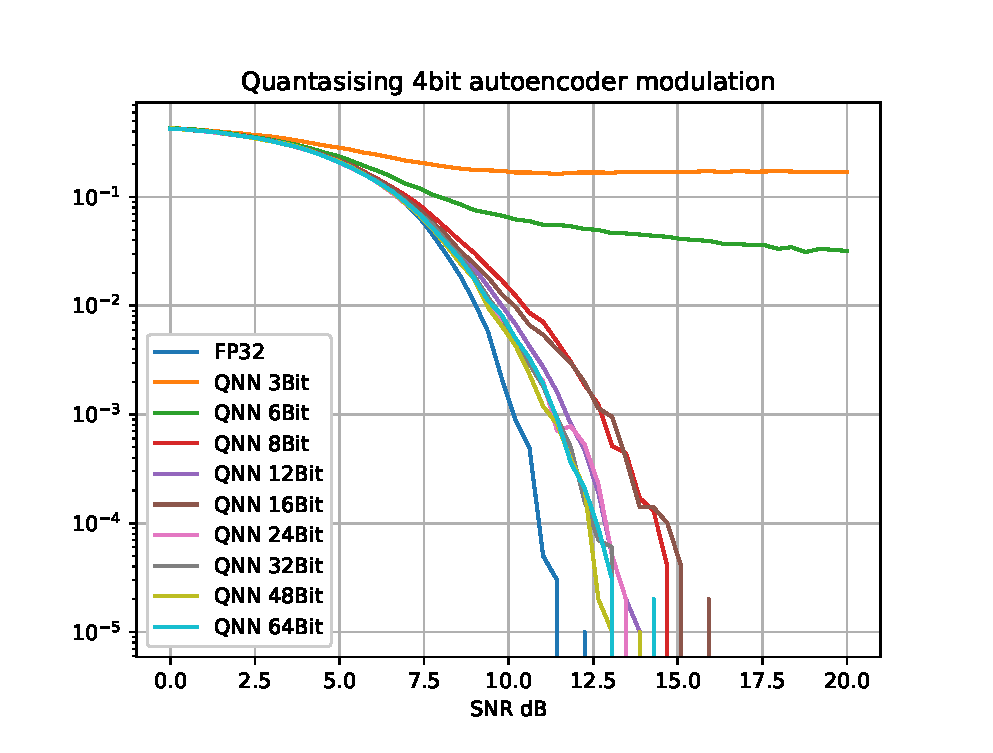
\includegraphics[width=0.85\textwidth]{autoencoder_qnn.eps}
	\caption{Autoencoder BER/SNR graph with post-training quantisation}
	\label{fig:qnn_snr}	
    \end{figure}
    
    \item \textbf{Other work in progress}\\
    We been facing an issue of autoencoder not being able to optimally assign symbols to bits. I been looking into making an algorithm that would do best effort mapping. Another method might also be working on a custom neural network cost function.
    Also been looking into binary neural networks (BNN) that use 1s and 0s for weights and activations as an alternative to QNN.
\end{itemize}



